\chapter{Analisi dei Requisiti}
\label{cap:analisi_requisiti}

\section{Panoramica e Attori}

L'obiettivo dello stage è lo sviluppo di un modulo di relying party (come definito nella sezione \ref{sec:dominio_applicativo}) che si occuperà di creare e inviare richieste standardizzate per ottenere attributi specifici degli utenti, gestire la ricezione dei VP Tokens tramite endpoint dedicati e verificare l'integrità delle presentazioni e la validità degli emettitori.

\subsection{Attori del sistema}
Gli attori rappresentano le entità (utenti fisici o sistemi esterni) che interagiscono con l'applicazione. Per il progetto sviluppato, sono stati individuati i seguenti attori principali:
\begin{itemize}
    \item \textbf{Relying Party:} rappresenta la componente backend del sistema che funge da entità richiedente e verificatrice delle Credenziali Verificabili. Gestisce l'intero ciclo di vita di una richiesta di presentazione: dall'inizializzazione della sessione, alla generazione del Request Object firmato crittograficamente, fino alla validazione delle presentazioni ricevute dal Wallet.
    \item \textbf{Wallet:} rappresenta un sistema esterno,tipicamente un'app mobile o un'estensione del browser, che custodisce le Credenziali Verificabili (Verifiable Credentials) emesse da uno o più Issuer fidati e le presenta su richiesta del Verifier. Nel contesto del protocollo OID4VP, il Wallet agisce come un intermediario tecnico tra l'Utente e il Relying Party: riceve la richiesta di presentazione, la interpreta, presenta all'Utente le credenziali richieste per ottenerne il consenso, e infine assembla e trasmette la Verifiable Presentation al Backend.
    \item \textbf{Utente finale:} è la persona fisica che interagisce con il sistema attraverso il Frontend del Relying Party e il proprio Wallet digitale. È il titolare delle Credenziali Verificabili, ovvero possiede documenti o attestazioni digitali (ad esempio un documento d'identità, una patente, un attestato professionale) emessi da Issuer fidati e memorizzati nel proprio Wallet. L'Utente rappresenta il soggetto che deve dimostrare il possesso di determinati attributi o qualifiche richieste dal servizio offerto dal Relying Party, ed è l'unico attore che può autorizzare la condivisione delle proprie credenziali.4
\end{itemize}

\subsection{Requisiti Obbligatori}
\begin{enumerate}
    \item \textbf{O01}: Inizializzazione della sessione di presentazione
    \item \textbf{O02}: Generazione dell'\textit{Authorization Request URL}
    \item \textbf{O03}: Esposizione dell'endpoint \texttt{request\_uri}
    \item \textbf{O04}: Pubblicazione dei metadati del Verifier (\texttt{client\_metadata})
    \item \textbf{O05}: Prevenzione degli attacchi di tipo \textit{replay}
    \item \textbf{O06}: Ricezione della risposta del Wallet
    \item \textbf{O07}: Validazione della struttura e dei criteri della \textit{DCQL Query}
    \item \textbf{O08}: Verifica della firma dell'Issuer (SD-JWT)
    \item \textbf{O09}: Verifica del \textit{Holder Binding} (KB-JWT)
    \item \textbf{O10}: Recupero della presentazione verificata
    \item \textbf{O11}: Gestione degli errori restituiti dal Wallet
    \item \textbf{O12}: Gestione della configurazione del client Relying Party tramite SCIM
\end{enumerate}
\subsection{Requisiti Desiderabili}
\begin{enumerate}
    \item \textbf{D01}: Supporto alla modalità di risposta \texttt{direct\_post.jwt} (JWE)
    \item \textbf{D02}: Generazione di chiavi effimere per la cifratura JWE
    \item \textbf{D03}: Risoluzione e verifica ricorsiva della \textit{Trust Chain}
    \item \textbf{D04}: Supporto a molteplici \textit{Client ID Scheme} (\texttt{redirect\_uri}, \texttt{x509\_san\_dns}, \texttt{x509\_hash}, \texttt{openid\_federation}, \texttt{verifier\_attestation}, \texttt{pre\_registered})
    \item \textbf{D05}: Esposizione dell'endpoint \texttt{/.well-known/openid-federation}
\end{enumerate}

\section{Casi d'uso}
I diagrammi dei casi d'uso (\textit{Use Case Diagram}) costituiscono una tipologia di diagrammi UML (\textit{Unified Modelling Language}) finalizzata a descrivere le interazioni tra gli attori del sistema e le funzionalità che quest'ultimo è chiamato a fornire.

Nelle sottosezioni seguenti vengono descritti nel dettaglio i casi d'uso relativi all'integrazione del modulo Relying Party nel sistema. Ciascun caso d'uso è presentato secondo la seguente struttura standardizzata:
\begin{itemize}
    \item \textbf{Caso d'uso:} codice identificativo e denominazione del caso d'uso;
    \item \textbf{Attori:} attori coinvolti nello scenario;
    \item \textbf{Descrizione:} descrizione dettagliata del caso d'uso, comprensiva dei passi che ne caratterizzano lo svolgimento;
    \item \textbf{Precondizioni:} condizioni che devono risultare soddisfatte affinché l'attore possa avviare il caso d'uso;
    \item \textbf{Postcondizioni:} stato del sistema al termine dell'esecuzione del caso d'uso;
    \item \textbf{Scenario principale:} sequenza ordinata di passi che descrivono il flusso nominale del caso d'uso, ossia la sequenza di azioni che si verifica in assenza di condizioni di errore;
    \item \textbf{Scenario alternativo:} eventuali flussi alternativi che possono verificarsi durante l'esecuzione del caso d'uso, con le relative condizioni di attivazione e le conseguenze sul sistema.
\end{itemize}

\begin{figure}[H]
    \centering
    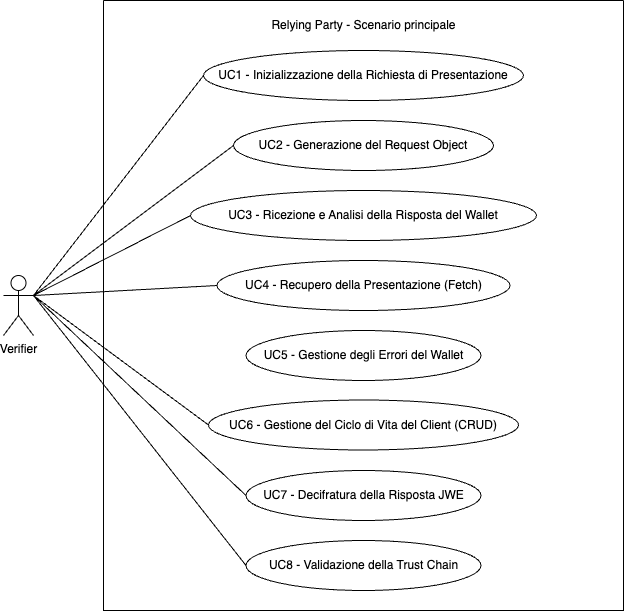
\includegraphics[width=0.7\textwidth]{./immagini/usecase/UC-Scenario Principale.png}    
    \caption{Diagramma dei casi d'uso -- Scenario principale del Relying Party}
    \label{fig:UC-Scenario Principale}
\end{figure}

\paragraph{\large\bfseries UC1: Inizializzazione della richiesta di presentazione}\mbox{}\\
\begin{figure}[H]
    \centering
    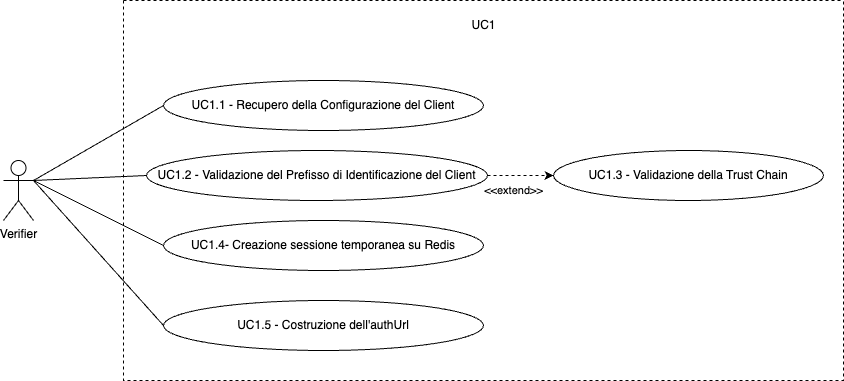
\includegraphics[width=0.7\textwidth]{./immagini/usecase/UC1.png}    
    \caption{UC1 -- Inizializzazione della richiesta di presentazione}
    \label{fig:UC1}
\end{figure}

\noindent\textbf{Attori:} Verifier, Utente finale.
\\
\textbf{Descrizione:} L'Utente finale, mediante l'interfaccia \textit{frontend} del Relying Party, avvia una nuova sessione di richiesta di presentazione di Credenziali Verificabili. Il Verifier procede alla validazione dell'identità del client precedentemente configurato, effettua — ove previsto dal \textit{Client ID Scheme} adottato — la verifica della \textit{Trust Chain} (nel caso di OpenID Federation), istanzia una sessione temporanea su Redis contenente la \textit{DCQL Query}, un \textit{nonce} crittografico e un identificativo univoco, e restituisce all'interfaccia \textit{frontend} un URL di autorizzazione (\texttt{authUrl}) e un identificativo di sessione (\texttt{sessionId}).
\\
\textbf{Precondizioni:}
\begin{itemize}
    \item Il client (Verifier) è stato precedentemente configurato nell'istanza MongoDB con parametri \texttt{redirectUris} e \texttt{vpFormatsSupported} validi.
    \item Il server Redis è raggiungibile e operativo.
    \item Le variabili d'ambiente del sistema sono configurate correttamente.
    \item Qualora il prefisso del \texttt{clientId} sia \texttt{openid\_federation}, la variabile d'ambiente \texttt{VERIFIER\_ENTITY\_IDENTIFIER} deve risultare impostata e le \textit{Trusted Authorities} devono essere raggiungibili.
    \item Qualora il prefisso sia \texttt{verifier\_attestation}, la variabile d'ambiente \texttt{VERIFIER\_ATTESTATION\_JWT} deve contenere un token JWT di attestazione valido.
\end{itemize}
\noindent\textbf{Postcondizioni:}
\begin{itemize}
    \item Una nuova sessione con stato \texttt{pending} è stata istanziata su Redis con un TTL (\textit{Time To Live}) configurato.
    \item La sessione contiene i seguenti parametri: \texttt{sessionId}, \texttt{requestId}, \texttt{nonce}, \texttt{transactionId}, \texttt{dcqlQuery}, \texttt{responseMode}, \texttt{prefixClientId}, \texttt{responseUri}.
    \item L'interfaccia \textit{frontend} ha ricevuto l'\texttt{authUrl} (contenente le informazioni necessarie al Wallet per elaborare la richiesta) e il \texttt{sessionId} (necessario per il successivo recupero della presentazione).
\end{itemize}

\noindent\textbf{Scenario principale:}
\begin{enumerate}
    \item L'Utente, mediante l'interfaccia \textit{frontend}, invia una richiesta HTTP \texttt{POST} all'endpoint \texttt{/init} con un payload contenente i parametri e \texttt{dcqlQuery}.
    \item Il Verifier recupera la configurazione del client dall'istanza MongoDB tramite i parametri \texttt{domainId} e \texttt{clientId}.
    \item Il Verifier valida il prefisso del \texttt{clientId}.
    \item Qualora il prefisso sia \texttt{openid\_federation}, il Client costruisce e valida la \textit{Trust Chain} verso il \textit{Trust Anchor} configurato.
    \item Il Verifier genera un \texttt{nonce}, un \texttt{requestId}, un \texttt{transactionId} e un \texttt{sessionId}.
    \item La sessione viene persistita su Redis.
    \item Il Verifier costruisce l'\texttt{authUrl}.
    \item Il Verifier restituisce una risposta HTTP \texttt{201 Created} con payload \texttt{\{success: true, sessionId, authUrl\}}.
\end{enumerate}

\noindent\textbf{Scenario alternativo:}
\begin{itemize}
    \item Qualora non risulti configurato alcun Verifier per il \texttt{domainId} fornito, il sistema solleva un'eccezione. Viene restituita una risposta HTTP \texttt{403 Forbidden}.
    \item Qualora il \texttt{TrustAnchorService} non riesca a costruire la \textit{Trust Chain}, il sistema solleva un'eccezione. Viene restituita una risposta HTTP \texttt{403 Forbidden}.
    \item Qualora non sia configurato l'url per il flusso \texttt{openid\_federation}, il sistema solleva un'eccezione. Viene restituita una risposta HTTP \texttt{400 Bad Request}.
    \item Qualora il prefisso fornito non sia valido, il sistema solleva un'eccezione. Viene restituita una risposta HTTP \texttt{501 Not Implemented}.
    \item Qualora il prefisso sia \texttt{verifier\_attestation} ma il token JWT non risulti valido, il sistema solleva un'eccezione. Viene restituita una risposta HTTP \texttt{400 Bad Request}.
\end{itemize}
\paragraph{\large\bfseries UC1.1: Verifica dell'identità del client configurato}
\label{uc:verifier:uc1.1}
\mbox{}\\
\noindent\textbf{Attori:} Verifier.
\\
\noindent\textbf{Descrizione:} Il Verifier recupera dall'istanza MongoDB la configurazione del client associato ai parametri \texttt{domainId} e \texttt{clientId} ricevuti nella richiesta HTTP. Tale configurazione comprende i parametri necessari per l'intero flusso di presentazione: \texttt{redirectUris}, \texttt{vpFormatsSupported}, \texttt{jwks} e gli algoritmi crittografici supportati.
\\
\noindent\textbf{Precondizioni:}
\begin{itemize}
    \item I parametri \texttt{domainId} e \texttt{clientId} sono stati forniti nella richiesta HTTP.
    \item L'istanza MongoDB è raggiungibile e operativa.
\end{itemize}
\noindent\textbf{Postcondizioni:}
\begin{itemize}
    \item L'oggetto \texttt{Client} è stato recuperato dall'istanza MongoDB.
\end{itemize}

\noindent\textbf{Scenario principale:}
\begin{enumerate}
    \item Il Verifier recupera la configurazione del client dal repository MongoDB.
    \item L'oggetto estratto dal repository viene validato e vengono verificati i campi obbligatori.
\end{enumerate}

\noindent\textbf{Scenario alternativo:}
\begin{itemize}
    \item Qualora nessun record corrisponda alla coppia \texttt{domainId}/\texttt{clientId} fornita, il sistema solleva un'eccezione e viene restituita una risposta HTTP \texttt{403 Forbidden}.
\end{itemize}

\paragraph{\large\bfseries UC1.2: Validazione del prefisso di identificazione del client}
\label{uc:verifier:uc1.2}
\mbox{}\\
\noindent\textbf{Attori:} Verifier.
\\
\noindent\textbf{Descrizione:} Il Verifier effettua il \textit{parsing} e la validazione del prefisso di identificazione del client (\texttt{prefixClientId}) al fine di determinare la modalità di autenticazione del Verifier nei confronti del Wallet.
\\
\noindent\textbf{Precondizioni:}
\begin{itemize}
    \item Il parametro \texttt{prefixClientId} è stato fornito nel corpo della richiesta HTTP; qualora risulti vuoto, viene applicato il valore predefinito \texttt{pre\_registered}.
    \item La configurazione del client è stata recuperata con successo (rif. \ref{uc:verifier:uc1.1}).
\end{itemize}
\noindent\textbf{Postcondizioni:}
\begin{itemize}
    \item Il prefisso è stato ricondotto a uno dei seguenti valori: \texttt{redirect\_uri}, \texttt{x509\_san\_dns}, \texttt{x509\_hash}, \texttt{openid\_federation}, \texttt{verifier\_attestation}, \texttt{pre\_registered}.
    \item Il risultato della validazione include i seguenti attributi: \texttt{clientIdValue}, \texttt{requiresSignature}, \texttt{headerExtensions}, \texttt{clientMetadataPolicy}.
\end{itemize}
\noindent\textbf{Scenario principale:}
\begin{enumerate}
    \item Il Verifier effettua il \textit{parsing} del valore del prefisso.
    \item In base al prefisso riconosciuto, il sistema applica la corrispondente logica di validazione:
    \begin{itemize}
        \item \texttt{redirect\_uri}: il valore \texttt{clientIdValue} viene costruito concatenando il prefisso al \texttt{responseUri} nella forma \texttt{redirect\_uri:<responseUri>}. Non è richiesta la firma crittografica del \textit{Request Object}. La politica sui metadati del client è impostata a \texttt{MUST\_INCLUDE}.
        \item \texttt{x509\_san\_dns}: dal JWKS del client viene estratta la catena certificativa \texttt{x5c} e viene validato il certificato \textit{leaf}. È richiesta la firma crittografica. La politica sui metadati è impostata a \texttt{MUST\_INCLUDE}.
        \item \texttt{x509\_hash}: dal JWKS viene estratta la catena \texttt{x5c} e viene calcolato il digest SHA-256 del certificato \textit{leaf}, utilizzato come identificativo del client. È richiesta la firma crittografica. La politica sui metadati è impostata a \texttt{MUST\_INCLUDE}.
        \item \texttt{openid\_federation}: come identificativo viene adottato il valore dell'\texttt{entityIdentifier}. È richiesta la firma crittografica. I metadati del client non devono essere inclusi nella richiesta (\texttt{MUST\_EXCLUDE}).
        \item \texttt{verifier\_attestation}: viene effettuato il \textit{parsing} del JWT di attestazione del Verifier, dal quale vengono estratti i claim \texttt{sub} e \texttt{cnf}. Il sistema verifica inoltre che il \texttt{responseUri} sia presente nella lista \texttt{redirect\_uris} contenuta nel JWT. È richiesta la firma crittografica. La politica sui metadati è impostata a \texttt{MUST\_INCLUDE}.
        \item \texttt{pre\_registered}: viene utilizzato direttamente il \texttt{clientId} già registrato nel sistema. Non è richiesta la firma crittografica. L'inclusione dei metadati è facoltativa (\texttt{NOT\_REQUIRED}).
    \end{itemize}
\end{enumerate}
\noindent\textbf{Scenario alternativo:}
\begin{itemize}
    \item Qualora il prefisso fornito sia \texttt{origin} viene restituita una risposta HTTP \texttt{501 Not Implemented}.
    \item Per i prefissi \texttt{x509\_san\_dns} e \texttt{x509\_hash}, qualora il JWKS del client non contenga una chiave di firma provvista di catena certificativa \texttt{x5c}, viene restituita una risposta HTTP \texttt{400 Bad Request}.
    \item Per il prefisso \texttt{x509\_san\_dns}, qualora nessun \texttt{dnsName} sia presente nel certificato corrisponda all'\textit{hostname} del \texttt{responseUri}, viene restituita una risposta HTTP \texttt{403 Forbidden}.
    \item Per il prefisso \texttt{verifier\_attestation}, qualora il JWT risulti privo dei claim \texttt{sub} o \texttt{cnf}, viene restituita una risposta HTTP \texttt{400 Bad Request}.
    \item Per il prefisso \texttt{verifier\_attestation}, qualora il \texttt{responseUri} non sia incluso nella lista \texttt{redirect\_uris} del JWT di attestazione, viene restituita una risposta HTTP \texttt{403 Forbidden}.
\end{itemize}

\paragraph{\large\bfseries UC1.3: Validazione della Trust Chain}
\label{uc:verifier:uc1.3}
\mbox{}\\
\noindent\textbf{Attori:} Verifier.
\\
\noindent\textbf{Descrizione:} Qualora il prefisso di identificazione del client sia \texttt{openid\_federation}, il sistema procede alla verifica della \textit{Trust Chain} dell'OpenID Provider, preliminarmente alla generazione della sessione.
\\
\noindent\textbf{Precondizioni:}
\begin{itemize}
    \item Il prefisso identificato nel caso d'uso UC1.2 (rif. \ref{uc:verifier:uc1.2}) è \texttt{openid\_federation}.
    \item La variabile d'ambiente \texttt{OPENID4VCI\_AUTHORIZE\_URL} è configurata e l'endpoint corrispondente è raggiungibile.
    \item Almeno un \textit{Trust Anchor} è specificato nel campo \texttt{trustedAuthorities} della \textit{DCQL Query}.
\end{itemize}
\noindent\textbf{Postcondizioni:}
\begin{itemize}
    \item L'appartenenza dell'OpenID Provider alla federazione di fiducia è stata confermata mediante la validazione completa della catena.
\end{itemize}
\noindent\textbf{Scenario principale:}
\begin{enumerate}
    \item Il sistema verifica la presenza della variabile d'ambiente \texttt{OPENID4VCI\_AUTHORIZE\_URL} e ne estrae l'\texttt{entityId} dell'OpenID Provider.
    \item Vengono estratte le \texttt{trustedAuthorities} dalla \textit{DCQL Query} fornita dall'interfaccia \textit{frontend}.
    \item Il Verifier avvia la costruzione e la validazione della \textit{Trust Chain} per l'\texttt{entityId} dell'OpenID Provider.
\end{enumerate}

\noindent\textbf{Scenario alternativo:}
\begin{itemize}
    \item Qualora la variabile d'ambiente non risulti configurata, viene restituita una risposta HTTP \texttt{400 Bad Request}.
    \item Qualora il \texttt{TrustAnchorService} rilevi una catena non valida, viene restituita una risposta HTTP \texttt{403 Forbidden}.
\end{itemize}

\paragraph{\large\bfseries UC1.4: Creazione della sessione temporanea su Redis}
\label{uc:verifier:uc1.4}
\mbox{}\\
\noindent\textbf{Attori:} Verifier.
\\
\noindent\textbf{Descrizione:} Il Verifier genera l'insieme degli identificativi crittografici necessari per la sessione e ne effettua la persistenza su Redis con un TTL (\textit{Time To Live}) configurabile.
\\
\noindent\textbf{Precondizioni:}
\begin{itemize}
    \item La validazione del prefisso è stata completata con successo (rif. \ref{uc:verifier:uc1.2}).
    \item Qualora il prefisso sia \texttt{openid\_federation}, la \textit{Trust Chain} è stata validata (rif. \ref{uc:verifier:uc1.3}).
    \item Il server Redis è raggiungibile e operativo.
\end{itemize}
\noindent\textbf{Postcondizioni:}
\begin{itemize}
    \item Una nuova sessione con stato \texttt{pending} è stata persistita su Redis, indicizzata mediante il \texttt{requestId} come chiave primaria.
    \item Il TTL è stato impostato.
\end{itemize}
\noindent\textbf{Scenario principale:}
\begin{enumerate}
    \item Il Verifier genera i seguenti identificativi crittografici:
    \begin{itemize}
        \item \texttt{requestId}: utilizzato come parametro \texttt{state} nel protocollo OID4VP.
        \item \texttt{nonce}: impiegato per la prevenzione degli attacchi di tipo \textit{replay}.
        \item \texttt{transactionId}: deputato al collegamento tra sessione e \textit{Response Record}.
        \item \texttt{sessionId}: restituito all'interfaccia \textit{frontend} per il successivo recupero della presentazione.
    \end{itemize}
    \item Viene istanziato l'oggetto \texttt{Session} con validazione dei campi obbligatori e verifica della conformità dei valori \texttt{nonce} e \texttt{requestId}.
    \item Il Client effettua la serializzazione dell'oggetto in formato JSON e ne esegue la persistenza su Redis con il TTL configurato.
\end{enumerate}
\noindent\textbf{Scenario alternativo:}
\begin{itemize}
    \item Qualora i valori \texttt{nonce} o \texttt{requestId} generati non superino la validazione di conformità viene restituita una risposta HTTP \texttt{400 Bad Request}.
\end{itemize}

\paragraph{\large\bfseries UC1.5: Costruzione dell'Authorization URL}\mbox{}\\
\noindent\textbf{Attori:} Verifier.
\\
\noindent\textbf{Descrizione:} Il Verifier costruisce l'URL di autorizzazione (\texttt{authUrl}) destinato a essere restituito all'interfaccia \textit{frontend} e successivamente presentato al Wallet mediante codice QR o \textit{deep link}.
\\
\noindent\textbf{Precondizioni:}
\begin{itemize}
    \item La sessione è stata creata con successo (rif.\ \ref{uc:verifier:uc1.4}).
    \item Il risultato della validazione del prefisso è disponibile (rif.\ \ref{uc:verifier:uc1.2}).
\end{itemize}
\noindent\textbf{Postcondizioni:}
\begin{itemize}
    \item L'\texttt{authUrl} è stato costruito nel formato conforme al tipo di prefisso adottato.
\end{itemize}
\noindent\textbf{Scenario principale:}
\begin{enumerate}
    \item Qualora la firma crittografica non sia richiesta: l'URL viene costruito utilizzando i seguenti \textit{query parameters}: \texttt{client\_id}, \texttt{response\_type=vp\_token}, \texttt{response\_mode}, \texttt{response\_uri}, \texttt{nonce}, \texttt{state} (corrispondente al \texttt{requestId}) e \texttt{dcql\_query}. Qualora la \texttt{clientMetadataPolicy} sia impostata a \texttt{MUST\_INCLUDE}, viene aggiunto il parametro \texttt{client\_metadata} contenente \texttt{vpFormatsSupported} e, opzionalmente, \texttt{jwks}.
    \item Qualora la firma crittografica sia richiesta: l'URL viene costruito includendo esclusivamente i parametri \texttt{client\_id}, \texttt{request\_uri} (puntante all'endpoint \texttt{/request/:requestId}) e \texttt{request\_uri\_method=post}.
\end{enumerate}

\section{Limiti}
